%load any "/usepackage" here...
\documentclass[journal = jpccck, manuscript = suppinfo]{achemso}
\setkeys{acs}{usetitle = true}
\usepackage{fixltx2e}
\usepackage{float}
\usepackage{achemso}
\usepackage{natbib}
\usepackage{multirow}
\usepackage{wrapfig}
\usepackage{times}
\usepackage{tablefootnote}
\usepackage{booktabs}
\usepackage[version=3]{mhchem}  % this is a great package for formatting chemical reactions
\usepackage{url}
\usepackage{graphicx}  % needed for figures
\usepackage{dcolumn}   % needed for some tables
\usepackage{bm}        % for math
\usepackage{amssymb}   % for math
\usepackage{booktabs}
\usepackage{tablefootnote}
\usepackage{mathptmx}

\newcommand*{\citen}[1]{%
  \begingroup
    \romannumeral-`\x % remove space at the beginning of \setcitestyle
    \setcitestyle{numbers}%
    \cite{#1}%
  \endgroup   
}


\title{Friction at ice-I$_\mathrm{h}$ / water interfaces is governed
  by solid-liquid hydrogen-bonding} 
\author{Patrick B. Louden}
\author{J. Daniel Gezelter} \email{gezelter@nd.edu}
\affiliation{Department of Chemistry and Biochemistry, University of
  Notre Dame, Notre Dame, IN 46556} 

\keywords{ice; water; interfaces; friction; hydrogen bonding}

\begin{document}

\section{Overview}
The supporting information contains further details about the model
construction, analysis methods, and supplies figures that support the
data presented in the main text.

\section{Fitting velocity profiles}
%%%%% All this goes in SI:
In order to calculate solid-liquid friction coefficients, $\kappa$
from Eq. (5) in the main text, the velocity profiles, $v_x(z)$,
obtained from each shearing simulation were fit assuming linear
behavior through each of the three regions of the simulation box; the
lower liquid, the solid, and the upper liquid. Parabolic functions
were designed to capture the negative slip behavior that links the
three regions,
\begin{equation}\label{vfit}
v(z) =
\begin{cases}
  v_{l} - m_{l}z & 0 \leq z < (z_{1} - w) \\
  v_{s} - \frac{1}{2}k(z-z_{1})^{2} & (z_{1}-w) \leq z < z_{1} \\
  v_{s}  & z_{1} \leq z < z_{2} \\
  v_{s} - \frac{1}{2}k(z-z_{2})^{2}  & z_{2} \leq z <( z_{2} + w)\\
  v_{s} - \frac{1}{2}kw^{2} - m_{l}(z-(z_{2} + w)) & (z_{2} + w) \leq z \\
\end{cases}
\end{equation}
  
Here, $v_{l}$ is the velocity of the liquid at the middle of the
liquid domain (the edge of the simulation box), and $v_{s}$ is the
velocity of the solid. The locations $z_{1}$ and $z_{2}$ are the edges
of the ice slab, and $w$ is the width of the interface (distinct from
$w_{10-90}$ mentioned in the main text). The parameter $m_{l}$ is the
slope of the velocity profile in the liquid regions of the box which
is related to the liquid-state viscosity. Figure \ref{fig:pyrComic}
shows a representative velocity profile (navy squares) and fit (green
line) with the locations of $z_{1}$ and $z_{2}$ indicated as vertical
dotted lines. Once the fits were obtained, the values for
$v_{x}(solid)$ and $v_{x}(liquid)$ for Eq. (5) were sampled from the
fit. The $z$ locations used to sample the fit were determined by
structural measures. The $z$ location for $v_{x}(liquid)$ was taken to
be the Gibbs dividing surface of the interface, less the 10$-$90 width
of the interface. Similarly, the $z$ location for $v_{x}(solid)$ was
taken to be the Gibbs dividing surface plus the 10$-$90 width of the
interface.

%The following 4 figures are the z-rnemd profiles a. q(z), b. T(z), c. Px(z)      \newpage 
\begin{figure}
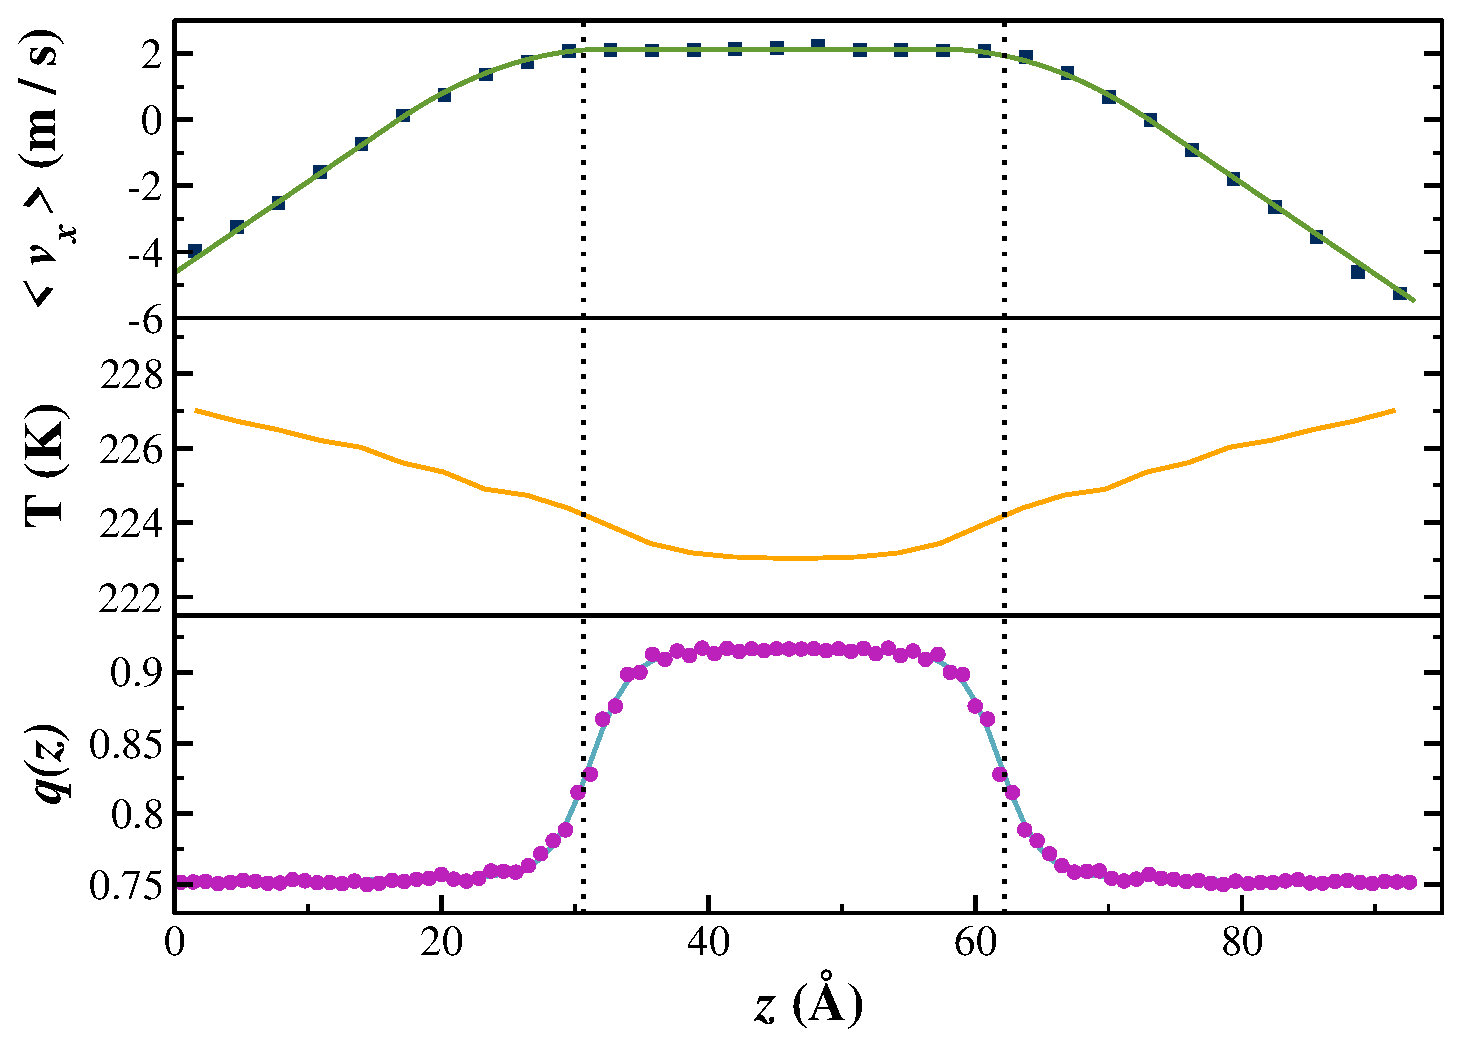
\includegraphics[width=\linewidth]{Pyr_comic_strip}
\caption{\label{fig:pyrComic} Properties of the pyramidal
  interface being sheared through water at 7.6
  ms\textsuperscript{-1}. Lower panel: the local tetrahedral order
  parameter, $q(z)$, (circles) and the hyperbolic tangent fit
  (turquoise line).  Middle panel: the imposed thermal gradient
  required to maintain a fixed interfacial temperature of 225 K. Upper
  panel: the transverse velocity gradient (squares) that develops in
  response to an imposed momentum flux, along with the fit (green
  line). The vertical dotted lines indicate the locations of the Gibbs
  dividing surfaces of the two interfaces.}
\end{figure}

\begin{figure}
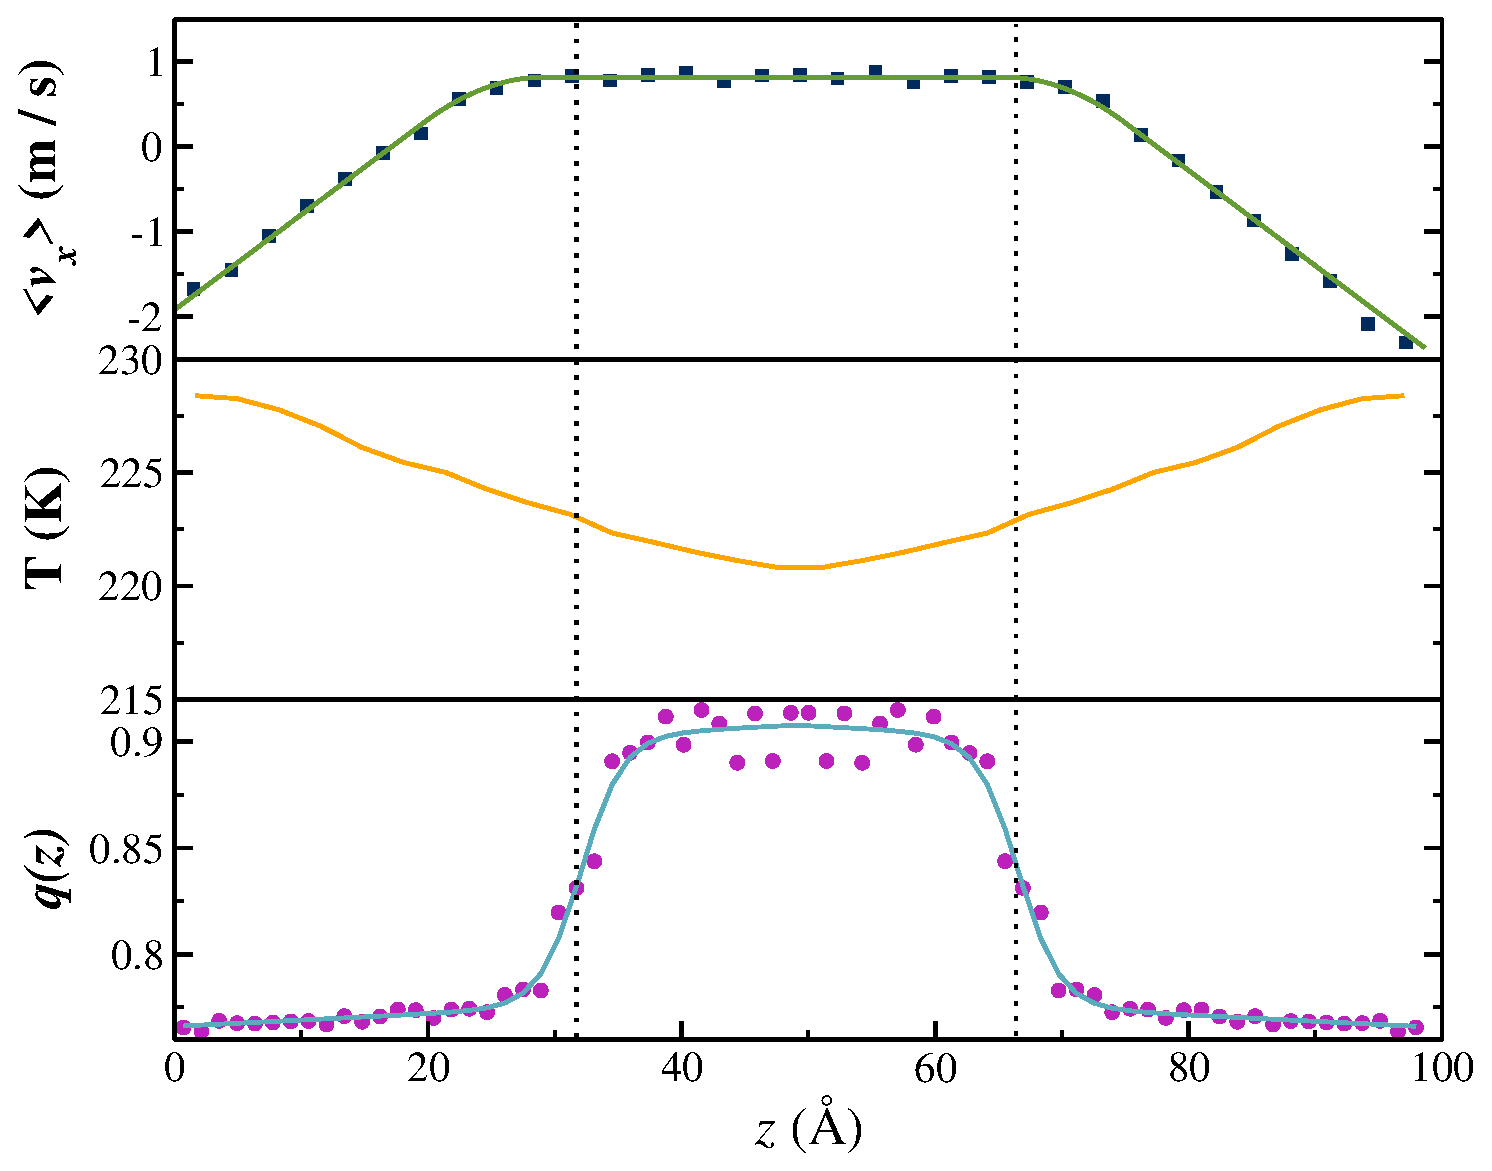
\includegraphics[width=\linewidth]{Bas_comic_strip}
\caption{\label{fig:bComic} Properties of the basal interface being
  sheared through water at 3.2 ms\textsuperscript{-1}.  Panel
  descriptions are the same as in Fig. \ref{fig:pyrComic}.}
\end{figure}

\begin{figure}
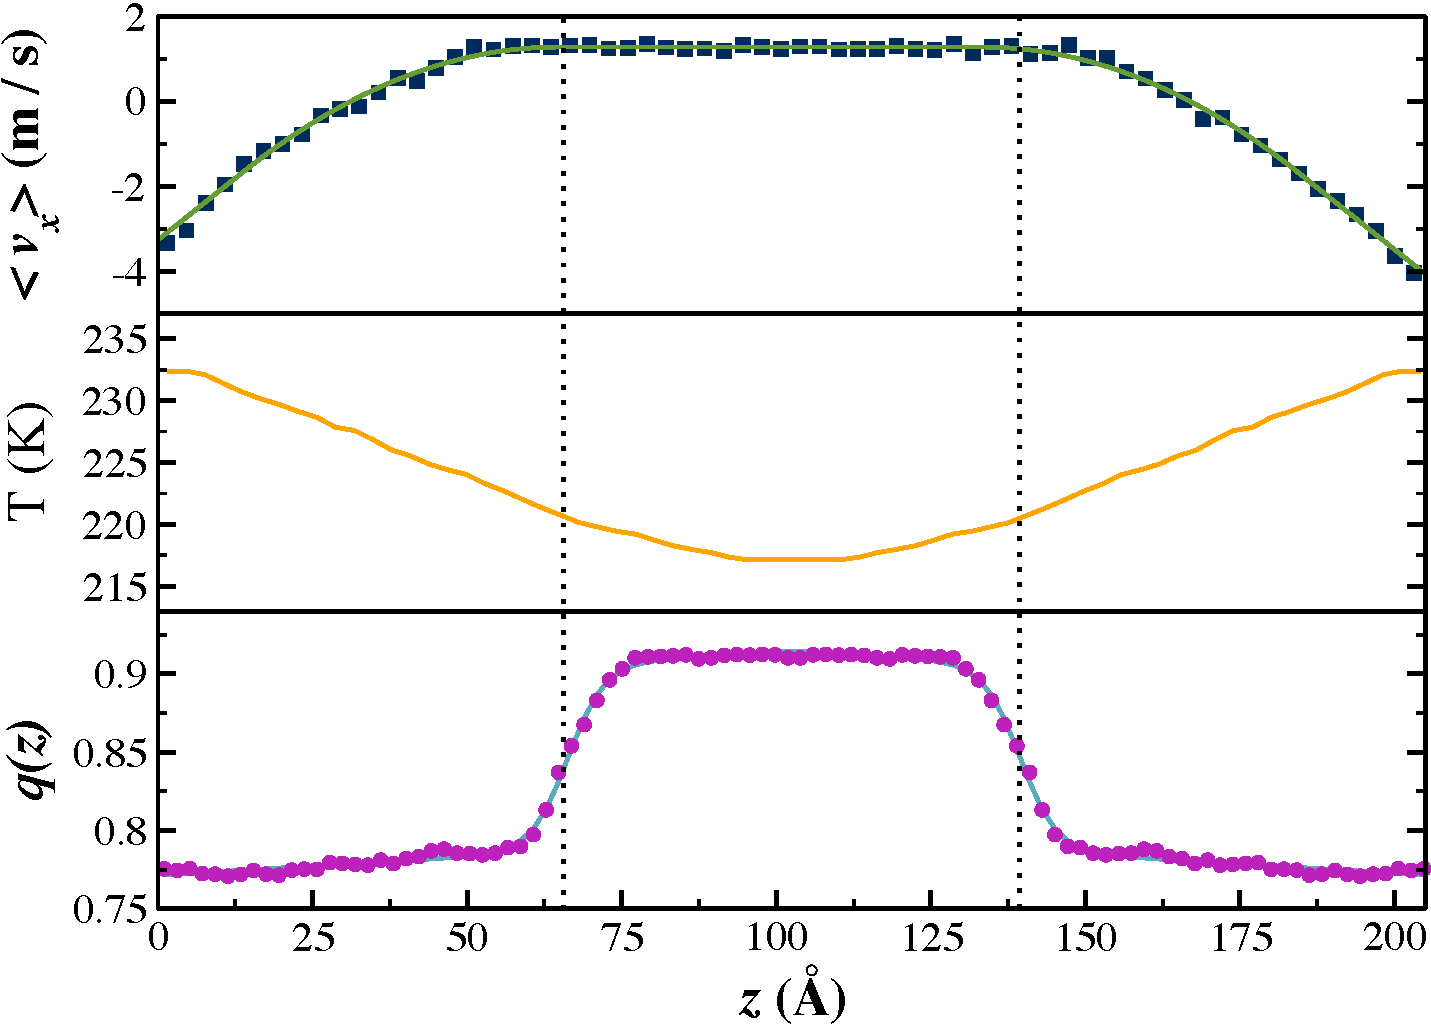
\includegraphics[width=\linewidth]{Pri_comic_strip}
\caption{\label{fig:pComic} Properties of the prismatic interface
  being sheared through water at 6.0 ms\textsuperscript{-1}.  Panel
  descriptions are the same as in Fig. \ref{fig:pyrComic}.}
\end{figure}
%End figures of z-rnemd profile. 


%Begin z-orientation times                                                         
\begin{figure}
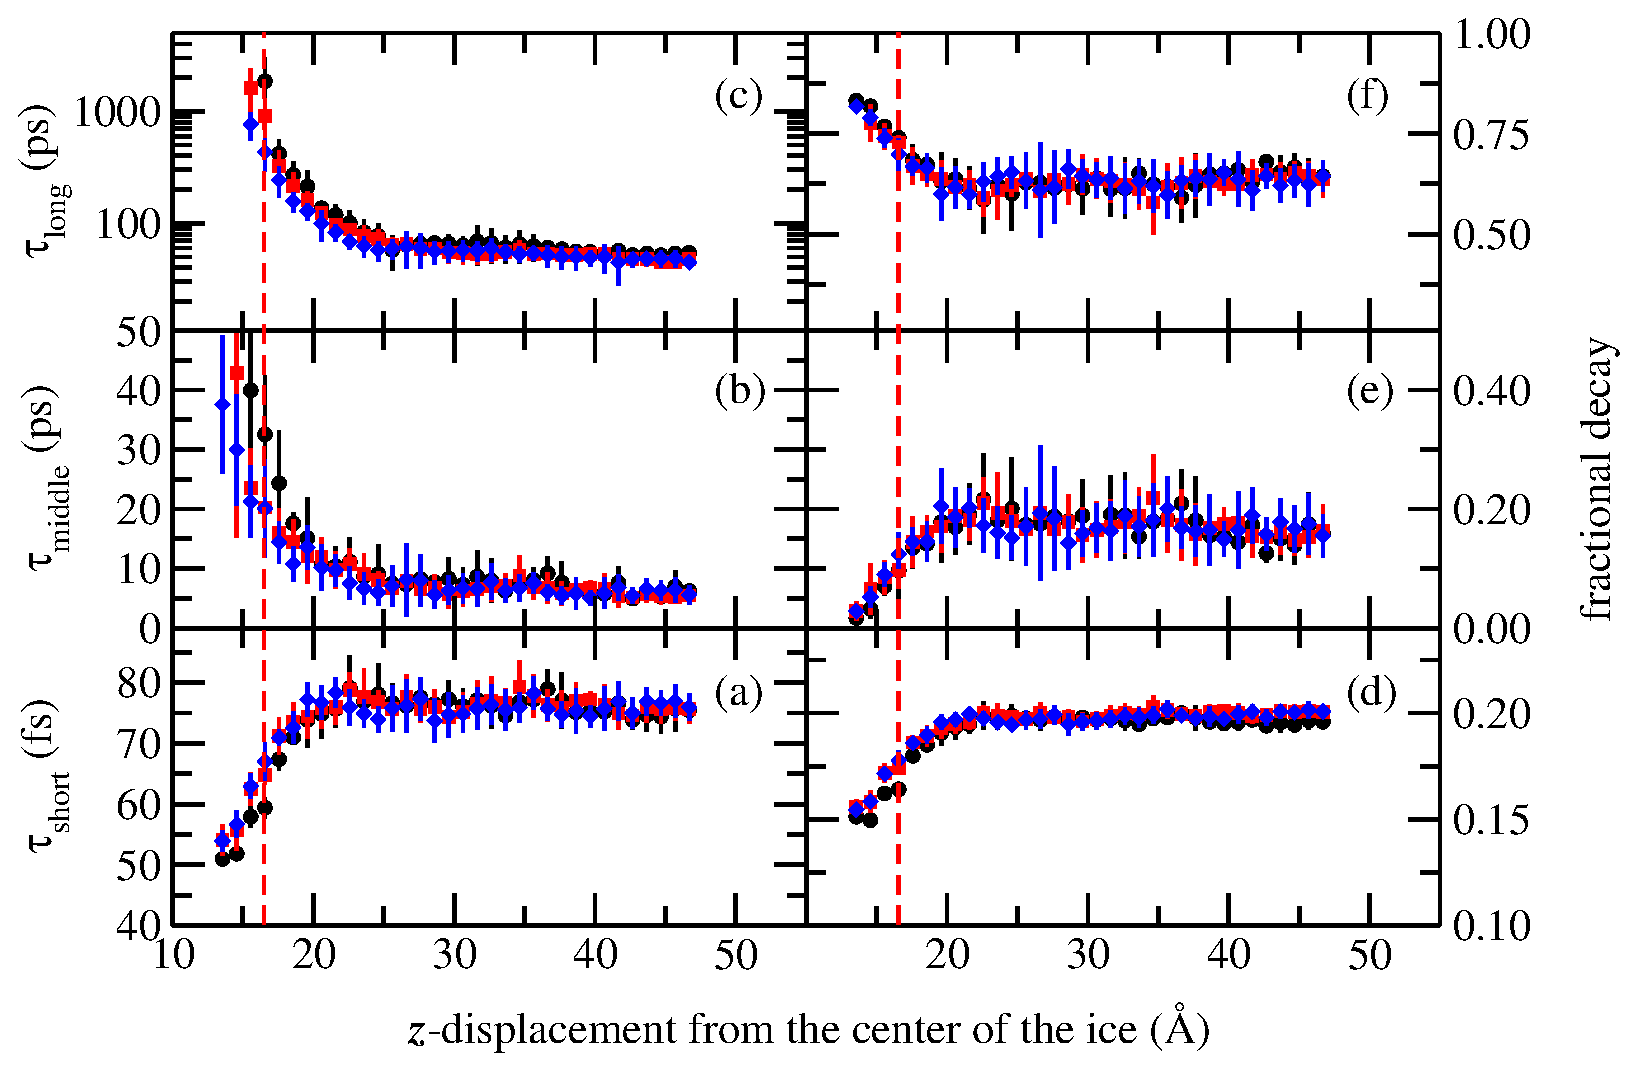
\includegraphics[width=\linewidth]{Pyr_lcorrz}
\caption{\label{fig:Pyrorient} Decay times (left) for $C_2(z,t)$ at
  the pyramidal interface, and their fractional contributions to the
  overall decay (right) fit using Eq. (8). The local decay constants
  are plotted as a function of distance from the center of the ice
  slab. The vertical dashed line indicates the Gibbs dividing surface
  determined using the local tetrahedral order parameter.  Results are
  shown for a quiescent system with no applied kinetic or momentum
  flux (black), an interface with with an imposed kinetic energy flux
  (red), and a sheared simulation (blue) with both kinetic and
  momentum fluxes.}
\end{figure}

\begin{figure}
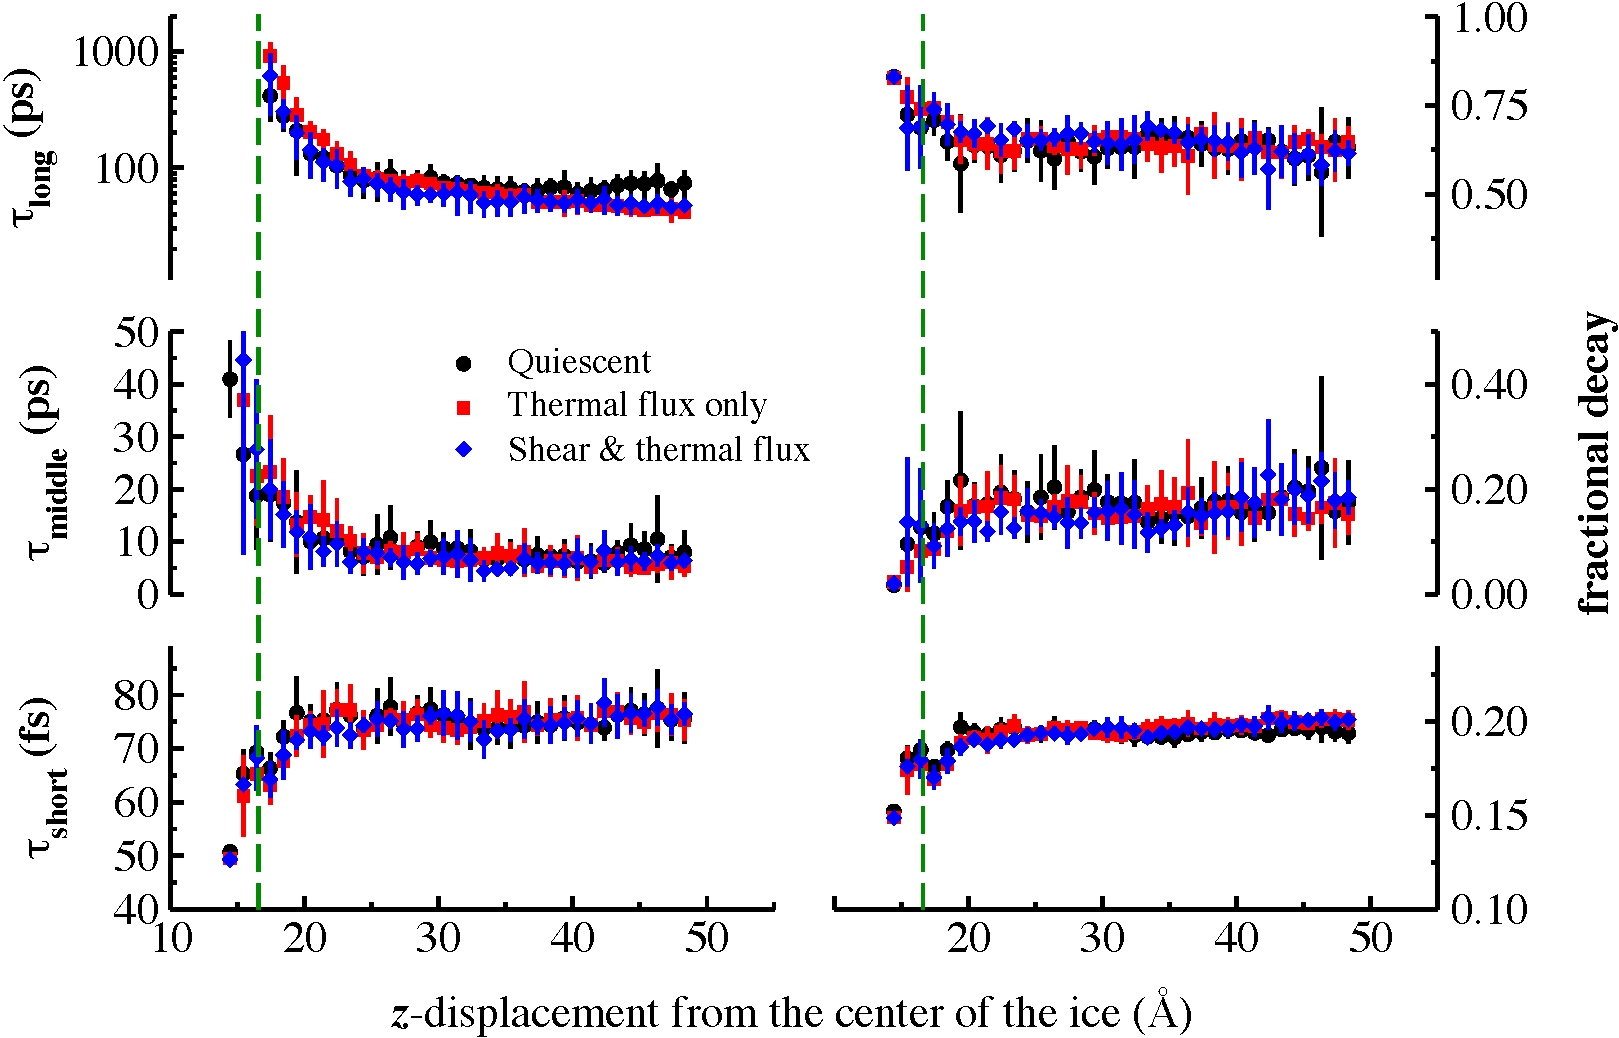
\includegraphics[width=\linewidth]{Bas_lcorrz}
\caption{\label{fig:Borient} $C_2(z,t)$ time constants for the basal
  interface.  Panel descriptions are the same as in
  Fig. \ref{fig:Pyrorient}. }
\end{figure}

\begin{figure}
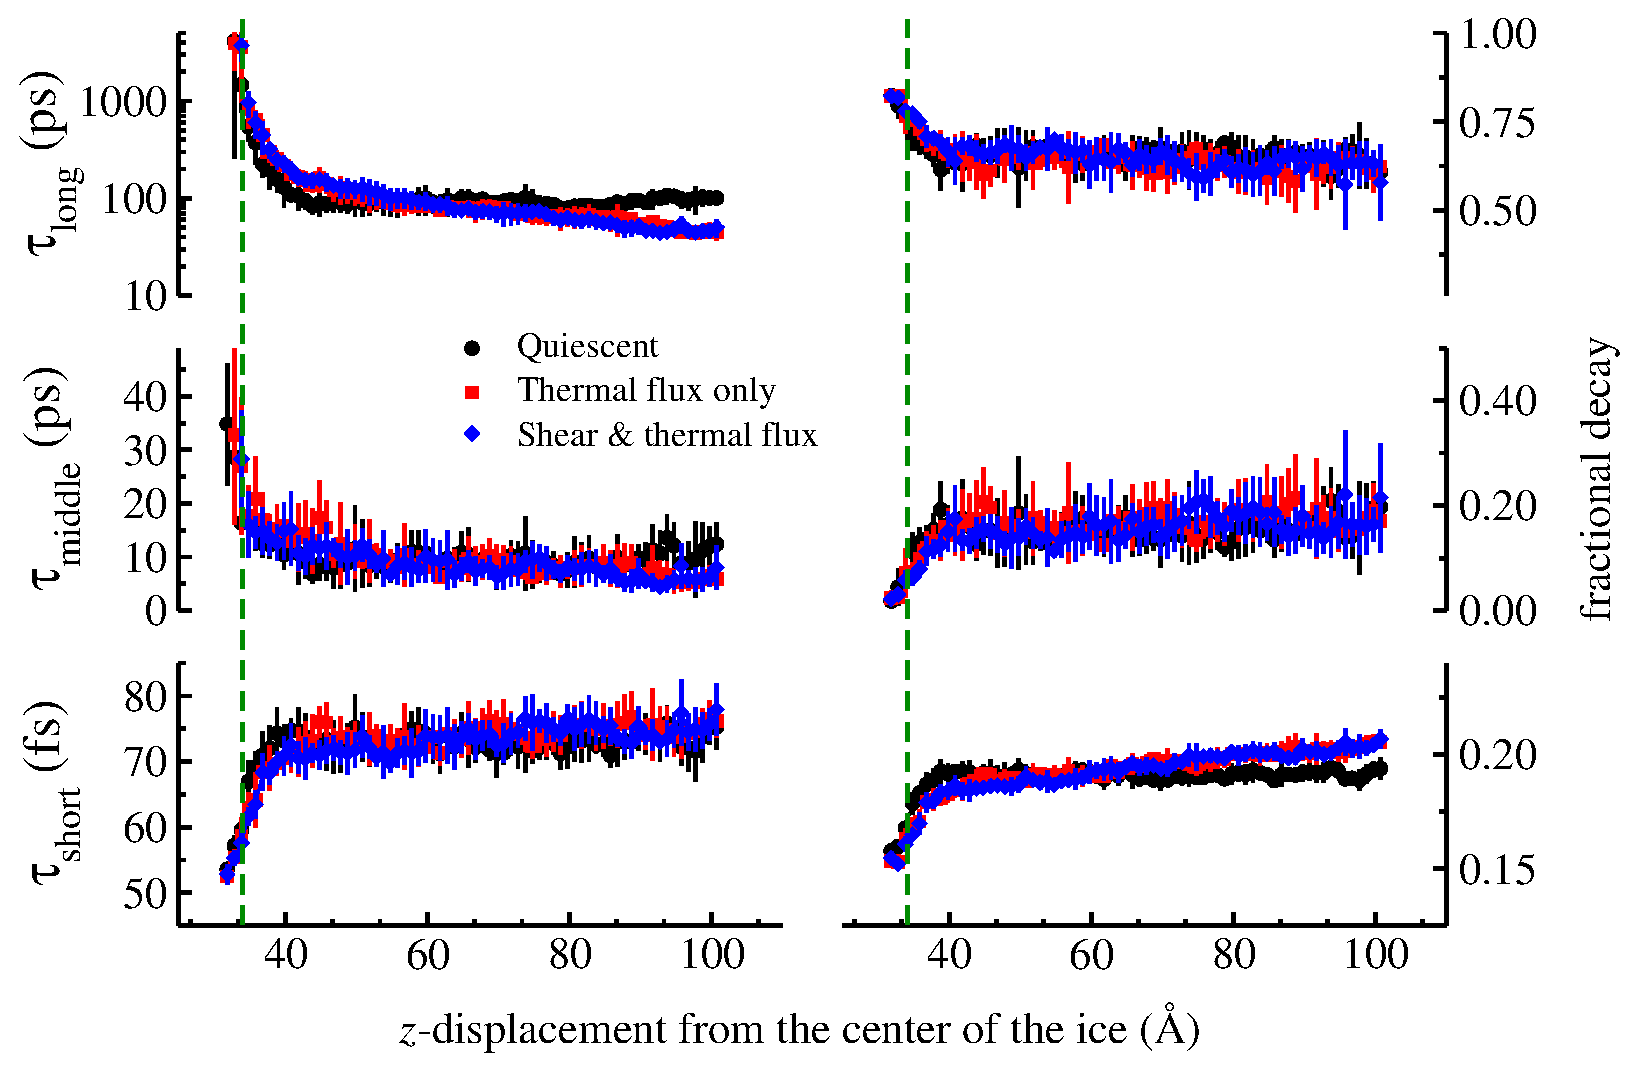
\includegraphics[width=\linewidth]{Pri_lcorrz}
\caption{\label{fig:Porient} $C_2(z,t)$ time constants for the prismatic
  interface.  Panel descriptions are the same as in
  Fig. \ref{fig:Pyrorient}.}
\end{figure}
%End z-orientation times                                                           
\begin{figure}
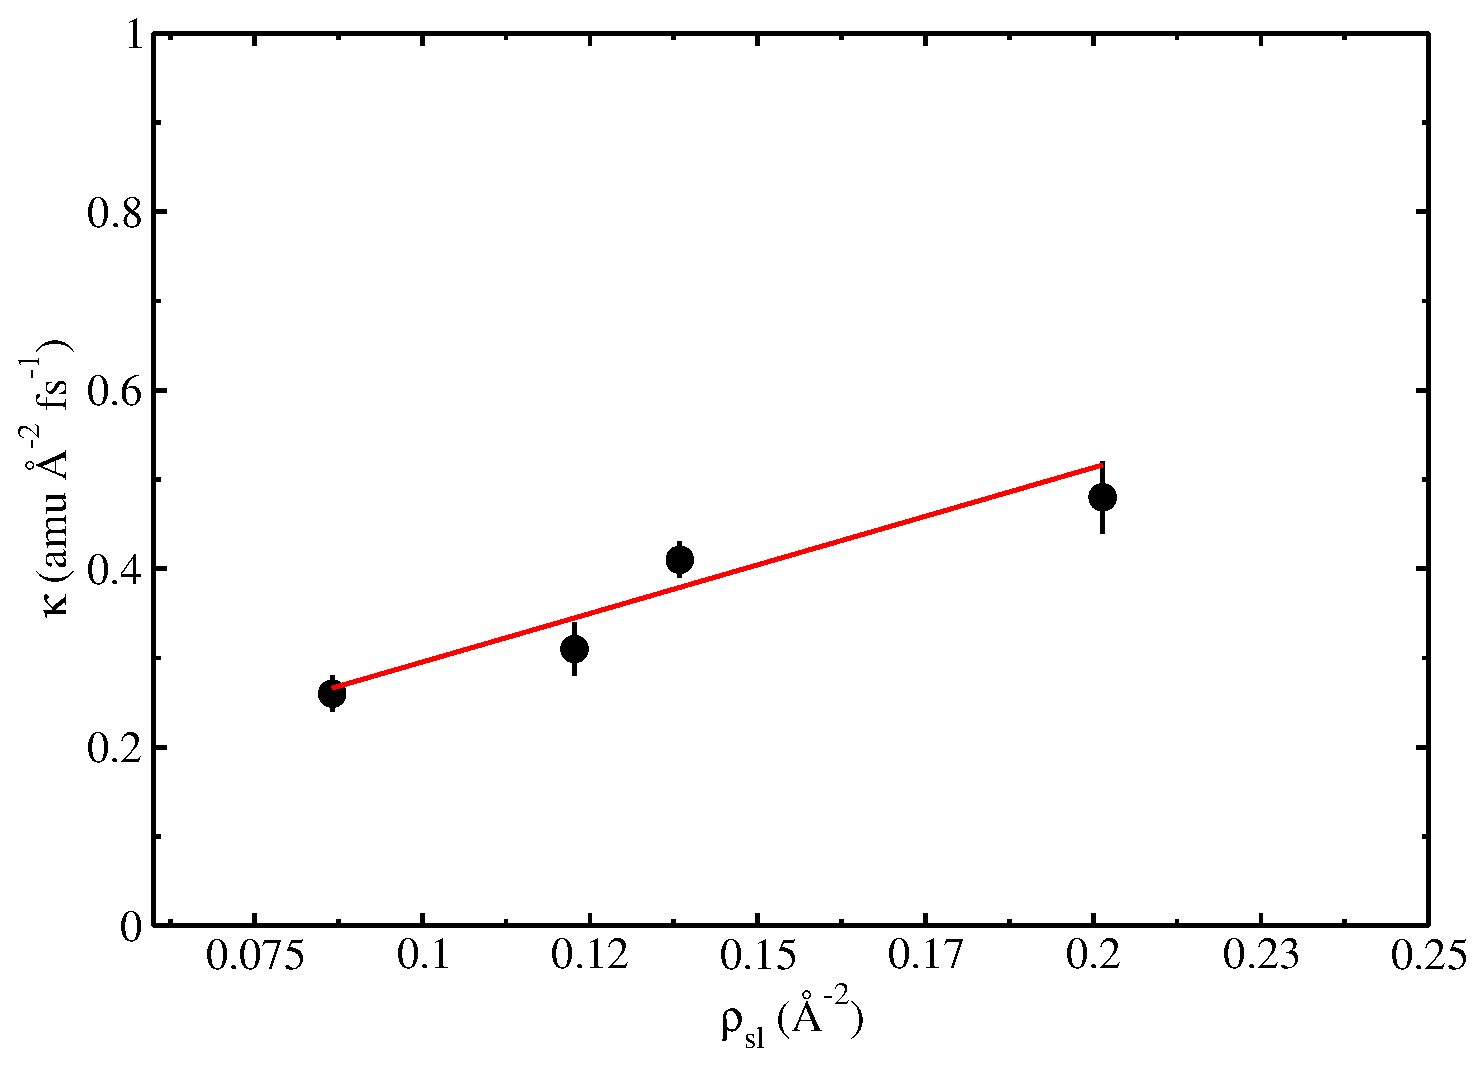
\includegraphics[width=\linewidth]{hb}
\caption{\label{fig:hbPlot} Solid-liquid friction coefficients by the
  surface density of hydrogen bonds. Linear regression gives a slope
  of 2.1772~(amu~fs\textsuperscript{-1}) and a y-intercept of
  0.0777~(amu~\AA\textsuperscript{-2}~fs\textsuperscript{-1}).} 
\end{figure}                                            


\end{document}
